\documentclass{llncs}
\usepackage{etex}

\usepackage{xcolor}
\usepackage{enumitem,amsmath,amssymb}
\usepackage{breakurl}    % used for \url and \burl
\usepackage[linesnumbered,boxed,noline,noend]{algorithm2e}
\def\defaultHypSeparation{\hskip.1in}

\usepackage{tikz}
\usepackage{subfig}
\usepackage{array,booktabs,multirow}
\usepackage{placeins}

\usepackage{logictools}
\usepackage{prooftheory}
\usepackage{comment}
\usepackage{mathenvironments}
\usepackage{drawproof}
\usepackage{bussproofs}
\usepackage{tensor}
\usepackage{mathtools}
\usepackage{amsmath}

\usepackage{graphicx}

\renewcommand{\topfraction}{0.85}
\renewcommand{\textfraction}{0.1}
\renewcommand{\floatpagefraction}{0.75}


\newcommand{\freevar}[1]{\mathrm{FV}(#1)}

\newcommand{\Vertices}[1]{V_{#1}}
\newcommand{\Edges}[1]{E_{#1}}
\newcommand{\Conclusion}[1]{\clause_{#1}}

\newcommand{\axiom}[1]{\widehat{#1}}
\newcommand{\n}{v}
\newcommand{\raiz}[1]{\rho(#1)}

\newcommand{\pedge}[3]{\ensuremath{\raiz{#1} \xrightarrow{#2} \raiz{#3}}}


\newcommand\inlineeqno{\stepcounter{equation}\ (\theequation)}


% Contraction
\newcommand{\con}[3]{\lfloor #1 \rfloor_{#2}^{#3}}

% Resolution
%\newcommand{\res}[6]{#1 \tensor[^{#2}_{#3}]{\odot}{^{#4}_{#5}} #6}
%\newcommand{\res}[6]{#1 \prescript{#2}{#3}{\odot^{#4}_{#5}} #6}

\newcommand{\res}[4]{\mathrel{\operatorname*{\odot}_{#1 #3}^{#2 #4}}}

\title{Towards the Compression of First-Order Resolution Proofs by Lowering Unit Clauses}

\author{
  Jan Gorzny\inst{1}
  \thanks{Supported by the Google Summer of Code 2014 program.}
  \and 
  Bruno Woltzenlogel Paleo\inst{2}
  \thanks{Supported by the Austrian Science Fund, project P24300.}
}

\authorrunning{J.\~Gorzny \and B.\~Woltzenlogel Paleo}

\institute{
  University of Victoria, Canada \\
  \email{jgorzny@uvic.ca}
  \and 
  Vienna University of Technology, Austria \\
  \email{bruno@logic.at}
}




\begin{document}

\maketitle


\begin{abstract}
The recently developed {\LowerUnits} algorithm compresses
propositional resolution proofs generated by SAT- and SMT-solvers by lowering (i.e. postponing) resolution inferences involving unit clauses (i.e. clauses having exactly one literal). This paper describes a generalization of this algorithm to the case of first-order resolution proofs generated by automated theorem provers. An empirical evaluation of a simplified version of this algorithm on hundreds of proofs shows promising results.
\end{abstract}


\setcounter{footnote}{0}

\section{Introduction}

Most of the effort in automated reasoning so far has been dedicated to the design and implementation of proof systems and efficient theorem proving procedures. As a result, saturation-based first-order automated theorem provers have achieved a high degree of maturity, with resolution \cite{Robinson} and superposition \cite{todo} being among the most common underlying proof calculi. Proof production is an essential feature of modern state-of-the-art provers and proofs are crucial for applications where the user requires certification of the answer provided by the prover. Nevertheless, efficient proof production is non-trivial \cite{SchultzAPPA}, and it is to be expected that the best, most efficient, provers do not necessarily generate the best, least redundant, proofs. And while the foundational problem of simplicity of proofs can be traced back at least to Hilbert's 24th Problem \cite{Hilbert}, the maturity of automated deduction has made it particularly relevant today. Therefore, it is a timely moment to develop methods that post-process and simplify proofs. 

For proofs generated by SAT- and SMT-solvers, which use propositional resolution as the basis for the DPLL and CDCL decision procedures, there is now a wide variety of proof compression techniques. Algebraic properties of the resolution
operation that might be useful for compression were investigated in \cite{bwp10}.
Compression algorithms based on rearranging and sharing chains of resolution inferences have been
developed in \cite{Amjad07} and \cite{Sinz}.  Cotton \cite{CottonSplit} proposed an algorithm that
compresses a refutation by repeteadly splitting it into a proof of a heuristically chosen literal $\ell$
and a proof of $\dual{\ell}$, and then resolving them to form a new refutation.  The {\ReduceReconstruct} algorithm \cite{RedRec} searches for locally redundant
subproofs that can be rewritten into subproofs of stronger clauses and with fewer resolution steps.
A linear time proof compression algorithm based on partial
regularization was proposed in \cite{RP08} and improved in \cite{LURPI}. Furthermore, \cite{LURPI} also described a new linear time algorithm called {\LowerUnits}, which delays resolution with unit clauses.

In contrast, for first-order theorem provers, there has been up to now (to the best of our knowledge) no attempt to design and implement an algorithm capable of taking a first-order resolution DAG-proof and efficiently simplifying it, outputting a possibly shorter pure first-order resolution DAG-proof. There are algorithms aimed at simplifying first-order sequent calculus tree-like proofs, based on cut-introduction \cite{BrunoLPAR,Hetzl}, and while in principle resolution DAG-proofs can be translated to sequent-calculus tree-like proofs (and then back), such translations lead to undesirable efficiency overheads. There is also an algorithm \cite{LPARCzech} that looks for terms that occur often in any TSTP \cite{TPTP} proof (including first-order resolution DAG-proofs) and introduces abbreviations for these terms. However, as the definitions of the abbreviations are not part of the output proof, it cannot be checked by a pure first-order resolution proof checker.

In this paper, we initiate the process of lifting propositional proof compression techniques to the first-order case, starting with the simplest known algorithm: {\LowerUnits} (described in Section \ref{sec:PropositionalLU}). As shown in Section \ref{sec:Challenges}, even for this simple algorithm, the fact that first-order resolution makes use of unification leads to many challenges that simply do not exist in the propositional case. In Section \ref{sec:FOLU} we describe a sophisticated algorithm that overcomes these challenges. Furthermore, in Section \ref{sec:SimpleFOLU} we describe a simpler version of this algorithm, which is easier to implement and possibly more efficient, at the cost of compressing less. In Section \ref{sec:exp} we present experimental results obtained by applying the simpler algorithm on hundreds of proofs generated with the {\SPASS} theorem prover \cite{SPASS}. The next section introduces the first-order resolution calculus using notations that are more convenient for describing proof transformation operations.






\section{The Resolution Calculus}

We assume that there are infinitely many variable symbols (e.g. $X$, $Y$, $Z$, $X_1$, $X_2$, \ldots), constant symbols (e.g. $a$, $b$, $c$, $a_1$, $a_2$, \ldots), function symbols of every arity (e.g $f$, $g$, $f_1$, $f_2$, \ldots) and predicate symbols of every arity (e.g. $p$, $q$, $p_1$, $p_2$,\ldots). A \emph{term} is any variable, constant or the application of an $n$-ary function symbol to $n$ terms.
An \emph{atomic formula} (\emph{atom}) is the application of an $n$-ary predicate symbol to $n$ terms. A \emph{literal} is an atom or the negation of an atom. The
\emph{complement} of a literal $\ell$ is denoted $\dual{\ell}$ (i.e. for any atom $p$,
$\dual{p} = \neg p$ and $\dual{\neg p} = p$). The set of all literals is denoted $\mathcal{L}$. A
\emph{clause} is a multiset of literals. $\bot$ denotes the \emph{empty clause}. A \emph{unit clause} is clause with a single literal. Sequent notation is used for clauses (i.e. $p_1,\ldots,p_n \seq q_1,\ldots, q_m$ denotes the clause $\{ \neg p_1,\ldots, \neg p_n, q_1, \ldots, q_m \}$).
$\freevar{t}$ (resp. $\freevar{\ell}$, $\freevar{\clause}$) denotes the set of variables in the term $t$ (resp. in the literal $\ell$ and in the clause $\clause$).
A \emph{substitution} $\{ X_1\backslash t_1, X_2 \backslash t_2, \ldots \}$ is a mapping from variables $\{ X_1, X_2, \ldots \}$ to, respectively, terms $\{t_1, t_2, \ldots \}$. The application of a substitution $\sigma$ to a term $t$, a literal $\ell$ or a clause $\clause$ results in, respectively, the term $t \sigma$, the literal $\ell \sigma$ or the clause $\clause \sigma$, obtained from $t$, $\ell$ and $\clause$ by replacing all occurrences of the variables in $\sigma$ by the corresponding terms in $\sigma$. The set of all substitutions is denoted $\mathcal{S}$. A \emph{unifier} of a set of literals is a substitution that makes all literals in the set equal.
A \emph{resolution proof} is a directed acyclic graph of clauses where the edges correspond to the inference rules of resolution and contraction (as explained in detail in Definition \ref{def:proof}). A \emph{resolution refutation} is a resolution proof with root $\bot$.


\begin{definition}[First-Order Resolution Proof] 
\label{def:proof} \hfill \\
A directed acyclic graph $\langle V, E, \clause \rangle$, where $V$ is a set of nodes and $E$ is a
set of edges labeled by literals and substitutions (i.e. $E \subset V \times \mathcal{L} \times \mathcal{S} \times V$ and $\n_1
\xrightarrow[\sigma]{\ell} \n_2$ denotes an edge from node $\n_1$ to node $\n_2$ labeled by the literal $\ell$ and the substitution $\sigma$), is a
proof of a clause $\clause$ iff it is inductively constructible according to the following cases:
%
\begin{itemize}
  \item \textbf{Axiom:} If $\Gamma$ is a clause, $\axiom{\Gamma}$ denotes some proof $\langle \{ \n \}, \varnothing,
    \Gamma \rangle$, where $\n$ is a new (axiom) node.
  \item \textbf{Resolution:} If $\psi_L$ is a proof $\langle V_L, E_L, \clause_L \rangle$ with $\ell_L \in \clause_L$ and
    $\psi_R$ is a proof $\langle V_R, E_R, \clause_R \rangle$ with $\ell_R \in \clause_R$, and 
    $\sigma_L$ and $\sigma_R$ are substitutions such that
    $\ell_L \sigma_L = \dual{\ell_R} \sigma_R$ and
    $\freevar{\left( \clause_L \setminus \left\{ \ell_L \right\} \right) \sigma_L} \cap 
     \freevar{\left( \clause_R
                    \setminus \left\{ \ell_R \right\} \right) \sigma_R} = \emptyset$, 
    then
    $\psi_L \res{\ell_L}{\sigma_L}{\ell_R}{\sigma_R} \psi_R$ denotes a proof $\langle V, E, \Gamma \rangle$ s.t.
    \begin{align*}
      V &= V_L \cup V_R \cup \{\n \} \\
      E &= E_L \cup E_R \cup
                    \left\{ \raiz{\psi_L} \xrightarrow[\sigma_L]{\ell_L} \n, 
                            \raiz{\psi_R} \xrightarrow[\sigma_R]{\ell_R} \n \right\} \\
     \Gamma &= \left( \clause_L \setminus \left\{ \ell_L \right\} \right) \sigma_L \cup \left( \clause_R
                    \setminus \left\{ \ell_R \right\} \right) \sigma_R 
    \end{align*}
    where $\n$ is a new (resolution) node and $\raiz{\varphi}$ denotes the root node of $\varphi$.
  \item \textbf{Contraction:} If $\psi'$ is a proof $\langle V', E', \clause' \rangle$ and $\sigma$ is a unifier of $\{\ell_1, \ldots \ell_n\}$ with $\{\ell_1, \ldots \ell_n\} \subseteq \clause'$, then, letting $\ell = \ell_k \sigma$ (for any $k \in \{1,\ldots, n\}$), $\con{\psi}{\sigma}{\ell}$ denotes a proof $\langle V, E, \Gamma \rangle$ s.t.
    \begin{align*}
      V &= V' \cup \{\n \} \\
      E &= E' \cup \{ \raiz{\psi'} \xrightarrow[\sigma]{\ell} \n \} \\
     \Gamma &= (\clause' \setminus \{ \ell_1, \ldots \ell_n \} ) \sigma \cup \{ \ell \}
    \end{align*}
    where $\n$ is a new (contraction) node and $\raiz{\varphi}$ denotes the root node of $\varphi$.
  \qed
\end{itemize}
\end{definition}




\noindent
If $\psi = \varphi_L \odot_{\ell} \varphi_R$, then $\varphi_L$ and $\varphi_R$ are \emph{direct
subproofs} of $\psi$ and $\psi$ is a \emph{child} of both $\varphi_L$ and $\varphi_R$. The
transitive closure of the direct subproof relation is the \emph{subproof} relation. A subproof which
has no direct subproof is an \emph{axiom} of the proof.
%
$\Vertices{\psi}$, $\Edges{\psi}$ and $\Conclusion{\psi}$
denote, respectively, the nodes, edges and proved clause (conclusion) of $\psi$.

\section{The Propositional LowerUnits Algorithm}
\label{sec:PropositionalLU}

We denote by $\dn{\psi}{\varphi_1, \varphi_2}$ the result of deleting the subproofs $\varphi_1$ and $\varphi_2$ from the proof $\psi$ and fixing it according to Algorithm \ref{algo:del}\footnote{
  The deletion algorithm is a minor variant of the \textsc{Reconstruct-Proof} algorithm presented in \cite{RP11}.
  The basic idea is to traverse the proof in a top-down manner, replacing
  each subproof having one of its premises marked for deletion (i.e. in $D$) by its other direct subproof. For more details, we refer to \ref{Boudou}.
}. 
We say that a subproof $\varphi$ in a proof $\psi$ can be lowered 
if there exists a proof
$\psi'$ such that $\psi' = \dn{\psi}{\varphi} \odot \varphi$ and
$\Conclusion{\psi'} \subseteq \Conclusion{\psi}$. If $\varphi$ originally participated in many resolution inferences within $\psi$ (i.e. if $\varphi$ had many children in $\psi$) then lowering $\varphi$ compresses the proof (in number of resolution inferences), because $\dn{\psi}{\varphi} \odot \varphi$ contains a single resolution inference involving $\varphi$.

%
It has been noted in \cite{LURPI} that, in the propositional case, $\varphi$ can always be lowered if it is a \emph{unit} (i.e. its conclusion clause is unit). This led to the invention of {\LowerUnits} (Algorithm \ref{algo:LU}), which aims at transforming a proof $\psi$ into $(\dn{\psi}{\mu_1,\ldots,\mu_n}) \odot_{\ell_1} \mu_1 \odot \ldots \odot_{\ell_n} \mu_n$, where $(\mu_1,\ldots,\mu_n)$ are all units with more than one child. Units with only one child are ignored merely because no compression is gained by lowering them. The order in which the units are reintroduced is important:
if a unit $\varphi_2$ is a subproof of a unit
$\varphi_1$ then $\varphi_2$ has to be reintroduced later than (i.e. below) $\varphi_1$.



\SetKwFunction{Rec}{delete}
\SetKw{Let}{let}

\begin{algorithm}[bt]
  \KwIn{a proof $\varphi$}
  \KwIn{$D$ a set of subproofs}
  \KwOut{a proof $\varphi'$ obtained by deleting the subproofs in $D$ from $\varphi$}
  \BlankLine

  \newcommand{\fixL}{\ensuremath{\varphi'_L}}
  \newcommand{\fixR}{\ensuremath{\varphi'_R}}

  \lIf{$\varphi \in D$ or $\raiz{\varphi}$ has no premises}{\Return{$\varphi$}}
  \BlankLine

  \Else{
    \Let{$\varphi_L$ and $\varphi_R$} be such that
      $\varphi = \varphi_L \res{\ell_L}{\sigma_L}{\ell_R}{\sigma_R} \varphi_R$ \;
    \Let{$\varphi'_L = $ \Rec{$\varphi_L$,$D$}} \;
    \Let{$\varphi'_R = $ \Rec{$\varphi_R$,$D$}} \;
    \BlankLine

    \lIf{$\varphi'_L \in D$}{ \Return{\fixR} }
    \lElseIf{$\varphi'_R \in D$}{ \Return{\fixL} }
    \BlankLine

    \lElseIf{$\dual{\ell} \notin \Conclusion{\fixL}$}{ \Return{\fixL} }
    \lElseIf{$\ell \notin \Conclusion{\fixR}$}{ \Return{\fixR} }
    \BlankLine

    \lElse{ \Return{ \fixL~$\res{\ell_L}{\sigma_L}{\ell_R}{\sigma_R}$~\fixR} }
  }

  \caption[.]{\FuncSty{delete}}
  \label{algo:del}
\end{algorithm}





A possible presentation of {\LowerUnits} is shown in Algorithm \ref{algo:LU}. Units are collected
during a first traversal. As this traversal is bottom-up, units are stored in a queue. The traversal
could have been top-down and units stored in a stack. Units are effectively deleted during a second,
top-down traversal. The last for-loop performs the reintroduction of units.

\begin{algorithm}[bt]
  \KwIn {a proof $\psi$}
  \KwOut{a compressed proof $\psi'$}
  \BlankLine

  \SetKwData{Units}{Units}
  \Units $\leftarrow \varnothing$ \;
  \BlankLine

  \For{every subproof $\varphi$ in a bottom-up traversal}{
    \If{$\varphi$ is a unit and has more than one child}{Enqueue $\varphi$ in \Units \; }
  }
  \BlankLine

  $\psi' \leftarrow $ \Rec{$\psi$,$\Units$} \;
  \BlankLine

  \For{every unit $\varphi$ in \Units}{
    \Let{$\{\ell\} = \Conclusion{\varphi}$} \;
    \lIf{$\dual{\ell} \in \Conclusion{\psi'}$}{
    $\psi' \leftarrow \psi' \odot_\ell \varphi$}
  }

  \caption{\LowerUnits}
  \label{algo:LU}
\end{algorithm}


\section{First-Order Challenges}\label{sec:Challenges}


In this section, we describe challenges that have to be overcome in order to successfully adapt {\RPI} to the first-order case. The first example illustrates the need to take unification into account. The other two examples discuss complex issues that can arise when unification is take into account in a naive way.

%straightforward example
\begin{example}\label{ex:unif} 
Consider the following irregular proof $\psi$. Naively computed, the safe literals for $\eta_3$ are $\{ \vdash q(c), ~ p(a,X)\}$. $\eta_1$ and $\eta_5$ and these two literals are unifiable. Further, the safe literals for $\eta_1$ includes $\eta_5$. Thus the proof can be regularized by recycling $\eta_1$.

\begin{footnotesize}
\begin{prooftree}
\def\e{\mbox{\ $\vdash$\ }}
\AxiomC{$\eta_1$: \e $p(W,X)$}
\AxiomC{$\eta_2$: $p(W,X)$ \e $q(c)$}
\BinaryInfC{$\eta_3$: \e $q(c)$}
\AxiomC{$\eta_4$: $q(c)$ \e $p(a,X)$}
\BinaryInfC{$\eta_5$: \e $p(a,X)$}
\AxiomC{$\eta_6$: $p(Y,b)$ \e }
\BinaryInfC{$\psi$: $\bot$}
\end{prooftree}
\end{footnotesize}

\noindent
Regularization of the proof by recycling $\eta_1$ results in deleting the edge between $\eta_2$ and $\eta_3$, which in turn replaces $\eta_3$ by $\eta_1$. Since $\eta_1$ cannot be resolved against $\eta_4$, and $\eta_1$ contained safe literals, $\eta_5$ is replaced by $\eta_1$. The result is the much shorter proof below.

\begin{footnotesize}
\begin{prooftree}
\def\e{\mbox{\ $\vdash$\ }}
\AxiomC{$\eta_1$: \e$p(W,X)$}
\AxiomC{$\eta_6$: $p(Y,b)$\e}
\BinaryInfC{$\psi'$: $\bot$}
\end{prooftree}
\end{footnotesize}

\noindent
Unlike in the propositional case, where the pivots and their corresponding safe literal list are all syntactically equal, in the first-order case, this is not necessarily the case. As illustrated above, $p(W,X)$ and $p(a,X)$ are not syntactically equal. Nevertheless, they are unifiable, and the proof can be regularized.
\end{example}

%unification necessary example
\begin{example}\label{ex:pairwise}

There are cases, as shown below, that require more careful care when attempting to regularize. Again, naively computed the safe literals for $\eta_3$ are $\{ \vdash q(c), ~ p(a,X)\}$, and so $\eta_1$ and $\eta_2$ appear to be candidates for regularization. 

\begin{footnotesize}
\begin{prooftree}
\def\e{\mbox{\ $\vdash$\ }}
\AxiomC{$\eta_1$: \e $p(a,c)$}
\AxiomC{$\eta_2$: $p(a,c)$ \e $q(c)$}
\BinaryInfC{$\eta_3$: \e $q(c)$}
\AxiomC{$\eta_4$: $q(c)$ \e $p(a,X)$}
\BinaryInfC{$\eta_5$: \e $p(a,X)$}
\AxiomC{$\eta_6$: $p(Y,b)$ \e }
\BinaryInfC{$\psi$: $\bot$}
\end{prooftree}
\end{footnotesize}


\noindent
However, if we attempt to regularize the proof, the same series of actions as in Example \ref{ex:unif} would result in the following resolution, which cannot be completed.

\begin{footnotesize}
\begin{prooftree}
\def\e{\mbox{\ $\vdash$\ }}
\AxiomC{$\eta_1$: \e$p(a,c)$}
\AxiomC{$\eta_6$: $p(Y,b)$\e}
\BinaryInfC{$\psi'$: ??}
\end{prooftree}
\end{footnotesize}

\end{example}

\noindent
The observations above lead to the idea of requiring pivots to satisfy the following property before collecting them to be reused.

\begin{definition}
\label{prop:pair}
Let $\eta$ be a clause with literal $\ell'$ with corresponding safe literal $\ell$ which is resolved against literals $\ell_1$, \ldots, $\ell_n$ in a proof $\psi$. $\eta$ is said to satisfy the \emph{pre-regularization unifiability property} in $\psi$ if $\ell_1$,\ldots,$\ell_n$, and $\dual{\ell'}$ are unifiable.
\end{definition}

\noindent
One technique to ensure this property is met is to apply the unifier of a resolution to each resolvent before computing the safe literals. In the case of Example \ref{ex:pairwise}, this would result in $\eta_1$ having the safe literals $\{ \vdash q(c),~p(a,b)\}$, and now it is clear that the literal in $\eta_1$ is not safe.

%TODO: continue from here
%extra check example
\begin{example}\label{ex:unifcheck}
Due to complications with unification, there are also cases where satisfying the pre-regularization unifiability property is not sufficient to attempt regularization. Consider the proof of $\psi$ below. After collecting the safe literals, $\eta_3$'s safe literals are $\{q(T,V),p(c,d)\vdash q(f(a,e),c)\}$.

\begin{footnotesize}
\begin{prooftree}
\def\e{\mbox{\ $\vdash$\ }}
\AxiomC{$\eta_8$: $q(f(a,e),c)\e$\hspace{-1cm}}
\AxiomC{$\eta_6$: $\e p(c,d)$\hspace{-4.5cm}}
\AxiomC{$\eta_1$: $p(U,V)\e q(f(a,V),U)$}
\AxiomC{$\eta_2$: $q(f(a,X),Y),q(T,X)\e q(f(a,Z),Y)$}
\BinaryInfC{$\eta_3$: $p(U,V),Q(T,V)\e q(f(a,Z),U)$\hspace{-3.5cm}}
\AxiomC{\hspace{-1.5cm} $\eta_4$: $\e q(R,S)$}
\BinaryInfC{$\eta_5$: $p(U,V)\e q(f(a,Z),U)$}
\BinaryInfC{$\eta_7$: $\e q(f(a,Z),c)$}
\BinaryInfC{$\psi$: $\bot$}
\end{prooftree}
\end{footnotesize}

\noindent
Since $q(f(a,X),Y) \in \eta_2$ and $q(T,V)$ (in $\eta_3$'s safe literals) are unifiable, regularization would be attempted. However, in this case, we would mark the edge between $\eta_2$ and $\eta_3$ for deletion, and as a result, $\eta_3$ will be replaced with $\eta_1$. $\eta_1$ does not contain the required pivot for $\eta_5$, and so $\eta_5$ is also replaced with $\eta_1$, and resolution is attempted before $\eta_1$ and $\eta_6$, which results in $\eta_7'$, and an inability to complete the proof, as shown below.

\begin{footnotesize}
\begin{prooftree}
\def\e{\mbox{\ $\vdash$\ }}
\AxiomC{$\eta_8$: $Q(f(ae)c)\e$}
\AxiomC{$\eta_6$: $\e P(cd)$}
\AxiomC{$\eta_1$: $P(UV)\e Q(f(aV)U)$}
\BinaryInfC{$\eta_7'$: $\e Q(f(ad)c)$}
\BinaryInfC{$\psi'$: ??}
\end{prooftree}
\end{footnotesize}

In order to avoid these scenarios, we perform an additional check during edge deletion. The node $\eta*$ which will replace a resolution $\eta$ (because $\eta$ would have a deleted parent), must be entirely contained, via unification which modifies only $\eta^*$'s variables, in the safe literals of $\eta$. In the case of this example, $\eta_1$ would not satisfy this property: in order to unify with $\eta_3$'s safe literals, it would be necessary to send $V\rightarrow Z$ due to $\eta_1$'s second literal, but leave $V$ unchanged due $\eta_1$'s first literal, which is not possible. Note that this check is not necessary in the propositional case, as the replacement node would be contained exactly in the set of safe literals.

\end{example}


%intersection example?


\section{First-Order LowerUnits} \label{sec:FOLU}

{\LowerUnits} does not lower every lowerable subproof. In particular, it does not take into
account the already lowered subproofs. For instance, if a unit $\varphi_1$ proving $\{a\}$ has
already been lowered, a subproof $\varphi_2$ with conclusion $\{\neg a, b\}$ may be lowered as well and
reintroduced above $\varphi_1$. The posterior reintroduction of $\varphi_1$ will resolve away $\neg a$ and guarantee that it does not occur in the resulting proof's conclusion. But care must also be taken not to lower $\varphi_2$ if $\neg a$ is a valent literal of
$\varphi_2$, otherwise $a$ will undesirably occur in the resulting proof's conclusion.

\begin{definition}[Univalent subproof]
A subproof $\varphi$ in a proof $\psi$ is \emph{univalent} w.r.t. a set $\Delta$ of literals iff
$\varphi$ has exactly one valent literal $\ell$ in $\psi$, $\ell \notin \Delta$ and
$\Conclusion{\varphi} \subseteq \Delta \cup \left\{ \ell \right\}$. $\ell$ is called the \emph{univalent
literal} of $\varphi$ in $\psi$ w.r.t.  $\Delta$.
\end{definition}

The principle of {\LowerUnivalents} is to lower all univalent subproofs. Having only one valent literal makes them behave essentially like units w.r.t. the technique of lowering. $\Delta$ is
initialized to the empty set. Then the complements of the univalent literals are incrementally added to
$\Delta$. Proposition \ref{prop:LUniv} ensures that the conclusion of the resulting proof
subsumes the conclusion of the original one.

\begin{proposition} \label{prop:LUniv}
Given a proof $\psi$, if 
%for an integer $n$
there is a sequence $U = (\varphi_1 \ldots \varphi_n)$
of $\psi$'s subproofs and a sequence $(\ell_1 \ldots \ell_n)$ of literals such that $\forall i \in
[1 \ldots n]$, $\ell_i$ is the univalent literal of $\varphi_i$ w.r.t. $\Delta_{i-1} =
\{\dual{\ell_1} \ldots \dual{\ell_{i-1}}\}$, then the conclusion of $$ \psi' = \dn{\psi}{U}
\odot_{\ell_n} \varphi_n \ldots \odot_{\ell_1} \varphi_1 $$ subsumes the conclusion of $\psi$.
\end{proposition}

\begin{proof}
The proposition is proven by induction on $n$, along with the fact that $\dn{\psi}{U} \notin U$.
For $n = 0$, $U = \varnothing$ and the properties trivially hold. Suppose a subproof
$\varphi_{n+1}$ of $\psi$ is univalent w.r.t. $\Delta_n$, with univalent literal $\ell_{n+1}$.
Because $\ell_{n+1} \notin \Delta_n$, there exists a subproof of $\dn{\psi}{U}$ with conclusion
containing $\dual{\ell_{n+1}}$, and therefore $\dn{\dn{\psi}{U}}{\varphi_{n+1}} \notin U \cup
\{\varphi_{n+1}\}$.  Let $\Gamma$ be the conclusion of $\dn{\psi}{U}$. The conclusion of $ \psi' =
\dn{\psi}{U \cup \{\varphi_{n+1}\}} = \dn{\dn{\psi}{U}}{\varphi_{n+1}} $ is included in $\Gamma \cup
\{\dual{\ell_{n+1}}\}$. The conclusion of $\psi' \odot_{\ell_{n+1}} \varphi_{n+1}$ is included in
$\Gamma \cup \Delta_n$. As $\Gamma \subseteq \Conclusion{\psi} \cup \Delta_n$, the conclusion of
$\psi' \odot_{\ell_{n+1}} \varphi_{n+1} \ldots \odot_{\ell_1} \varphi_1$ is included in
$\Conclusion{\psi}$. \qed
\end{proof}

For this principle to lead to proof compression, it is important to take care
of the mutual inclusion of univalent subproofs.
%not only of the order in which subproofs are collected for lowering but also of deleting all
%already collected univalent subproofs from the next subproof $\psi_i$ before reintroducing it.
Suppose, for instance, that $\varphi_i, \varphi_j, \varphi_k \in U$, $i < j < k$, $\varphi_j$ is a
subproof of $\varphi_i$ but not a subproof of $\dn{\psi}{\varphi_i}$, and $\dual{\ell_j} \in
\Conclusion{\varphi_k}$.  In this case, $\varphi_j$ will have one more child in
$$
\dn{\psi}{U} \odot_{\ell_n} \varphi_n \ldots \odot_{\ell_k} \varphi_k \ldots \odot_{\ell_j} \varphi_j \ldots \odot_{\ell_i} \varphi_i \ldots \odot_{\ell_1} \varphi_1
$$
than in the original proof $\psi$. The additional child is created when $\varphi_j$ is reintroduced.
All the other children are reintroduced with the reintroduction of $\varphi_i$, because
$\varphi_j$ was not deleted from $\varphi_i$.

To solve this issue, {\LowerUnivalents} traverses the proof in a top-down manner and simultaneously
deletes already collected univalent subproofs, as sketched in Algorithm \ref{algo:LUniv}.  


\SetKwData{Univ}{Univalents}
\begin{algorithm}[bt]
  \KwIn {a proof $\psi$}
  \KwOut{a compressed proof $\psi'$}
  \BlankLine

  \SetKw{Push}{push}
  \SetKw{Pop} {pop}

  \Univ $\leftarrow \varnothing$ \;
  $\Delta \leftarrow \varnothing$ \;
  \BlankLine

  \For{every subproof $\varphi$, in a top-down traversal \label{line:LUniv:step1begin} }{
    $\psi' \leftarrow$ \Rec{$\varphi$,\Univ} \label{line:LUniv:delete} \;
    \If{$\psi'$ is univalent w.r.t. $\Delta$ \label{line:LUniv:lunivtest} }{
      \Let{$\ell$} be the univalent literal \;
      \Push $\dual{\ell}$ onto $\Delta$ \label{line:LUniv:pushDelta} \;
      \Push $\psi'$     onto \Univ \label{line:LUniv:step1end} \;
    }
  }
  \BlankLine

  \tcp{At this point, $\psi' = \dn{\psi}{\Univ}$}
  \While{\Univ $\neq \varnothing$}{ \label{line:LUniv:reintroducebegin}
    $\varphi \leftarrow$ \Pop from \Univ \;
    $\ell \leftarrow$ \Pop from $\Delta$ \;
    \lIf{$\ell \in \Conclusion{\psi'}$ \label{line:LUniv:testreintroduce} }{
    $\psi' \leftarrow \varphi \odot_\ell \psi'$ \;}
  }

  \caption{Simplified \LowerUnivalents}
  \label{algo:LUniv}
\end{algorithm}


Figure \ref{fig:exluniv} shows an example proof and the result of compressing it with \LowerUnivalents. The top-down traversal starts with the leaves (axioms) and only visits a child when all its parents have already been visited. Assuming the unit with conclusion $\{a\}$ is the first visited leaf, it passes the univalent test in line \ref{line:LUniv:lunivtest}, is marked for lowering (line \ref{line:LUniv:step1end}) and the complement of its univalent literal is pushed onto $\Delta$ (line \ref{line:LUniv:pushDelta}). When the subproof with
conclusion $\{\dual{a},b\}$ is considered, $\Delta = \{\dual{a}\}$. As this subproof has only one
valent literal $b \notin \Delta$ and $\{\dual{a},b\} \subseteq \Delta \cup \{b\}$, it is
marked for lowering as well. At this point, $\Delta = \{\dual{a}, \dual{b}\}$, \texttt{Univalents} contains the two subproofs marked for lowering and $\psi'$ is the subproof with conclusion $\{\dual{a}, \dual{b}\}$ shown in Subfig. (b) (i.e. the result of deleting the two marked subproofs from the original proof in Subfig. (a)). No other subproof is univalent; no other subproof is marked for lowering. The final compressed proof (Subfig. (b)) is obtained by reintroducing the two univalent subproofs that had been marked (lines \ref{line:LUniv:reintroducebegin} -- \ref{line:LUniv:testreintroduce}). It has one resolution less than the original. This is so because the subproof with conclusion $\{\dual{a},b\}$ had been used (resolved) twice in the original proof, but lowering delays its use to a point where a single use is sufficient.

\begin{figure}[htb]
  \centering
  \subfloat[Original proof]{
    \centering
    \begin{tikzpicture}

      \rootnode;
      \withchildren{root} {r0}{\dual{a}}  {unit}{a};
      \withchildren{r0}   {r1}{\dual{a},c} {r2}{\dual{a},\dual{c}};
      \withchildren{r1}   {a0}{\dual{b},c} {low}{\dual{a},b};

      \proofnode[above right of=r2] {a1} {\dual{a},\dual{b},\dual{c}};
      \drawchildren {r2} {low} {a1};

    \end{tikzpicture}
  } \qquad
  \centering
  \subfloat[Compressed proof]{
    \centering
    \begin{tikzpicture}

      \rootnode;
      \withchildren{root} {r0}{\dual{a}}          {unit}{a};
      \withchildren{r0}   {r1}{\dual{a},\dual{b}} {low}{\dual{a},b};
      \withchildren{r1}   {a0}{\dual{b},c}        {a1}{\dual{a},\dual{b},\dual{c}};

    \end{tikzpicture}
  }
\caption{Example of proof crompression by \LowerUnivalents} 
\label{fig:exluniv}
\end{figure}


% Discussion of optimizations follow

Although the
call to \FuncSty{delete} inside the first loop (line \ref{line:LUniv:step1begin} to
\ref{line:LUniv:step1end}) suggests quadratic time complexity, this loop (line
\ref{line:LUniv:step1begin} to \ref{line:LUniv:step1end}) can be (and has been) actually implemented
as a recursive function extending a recursive implementation of \FuncSty{delete}. With such an
implementation, {\LowerUnivalents} has a time complexity linear w.r.t. the size of the proof, assuming the
univalent test (at line \ref{line:LUniv:lunivtest}) is performed in constant bounded time. 


Determining whether a literal is valent is expensive. But thanks to Proposition \ref{prop:valentactive},
subproofs with one active literal which is not in $\Conclusion{\psi}$ can be considered instead
of subproofs with one valent literal.  If the active literal is not valent, the corresponding
subproof will simply not be reintroduced later (i.e. the condition in line 28 of Algorithm \ref{algo:fullLUniv} will fail).

While verifying if a subproof could be univalent, some edges might be deleted. If a
subproof $\varphi_i$ has already been collected as univalent subproof with univalent literal
$\ell_i$ and the subproof $\varphi'$ being considered now has $\ell_i$ as active literal, the
corresponding incoming edges can be removed. Even if $\ell_i$ is valent for $\varphi'$, only
$\dual{\ell_i}$ would be introduced, and it would be resolved away when reintroducing
$\varphi_i$. The \FuncSty{delete} operation can be easily modified to remove both nodes and edges.

Algorithm \ref{algo:fullLUniv} sums up the previous remarks for an efficient implementation of
{\LowerUnivalents}. As noticed above, sometimes this algorithm may consider a subproof as univalent when it
is actually not. But as care is taken when reintroducing subproofs (at line \ref{line:full:testreintroduce}),
the resulting conclusion still subsumes the original.  The test that $\ell \in \Conclusion{\varphi}$
at line \ref{line:full:testactive} is mandatory since $\ell$ might have been deleted from
$\Conclusion{\varphi}$ by the deletion of previously collected subproofs.

\begin{algorithm}[pbt]
  \SetAlgoVlined
  \SetAlgoShortEnd

  \KwData {a proof $\psi$, compressed in place}
  \KwIn {a set $D_V$ of subproofs to delete}
  \KwIn {a set $D_E$ of edges to delete}
%  \KwOut{the proof $\psi$ compressed in place}
  \BlankLine

  \SetKw{Push}{push}
  \SetKw{Pop} {pop}
  \SetKw{Add} {add}
  \SetKw{Rep} {replace}

  \SetKwData{Activ}{ActiveLiterals}

  \Univ $\leftarrow \varnothing$ \;
  $\Delta \leftarrow \varnothing$ \;
  \BlankLine

  \For{every subproof $\varphi$, in a top-down traversal of $\psi$ }{

    \tcp{The deletion part.}
    \If{$\varphi$ is not an axiom}{
      \Let{$\varphi = \varphi_L \odot_\ell \varphi_R$} \;
      \uIf{ $\varphi_L \in D_V$ or $\pedge{\varphi}{\dual{\ell}}{\varphi_L} \in D_E$ }{
        \uIf{ $\pedge{\varphi}{\ell}{\varphi_R} \in D_E$ }{
          \Add $\varphi$ to $D_V$ \;
        }
        \Else{
          \Rep $\varphi$ by $\varphi_R$ \;
        }
      }
      \ElseIf{ $\varphi_R \in D_V$ or $\pedge{\varphi}{\dual{\ell}}{\varphi_R} \in D_E$ }{
        \uIf{ $\pedge{\varphi}{\ell}{\varphi_L} \in D_E$ }{
          \Add $\varphi$ to $D_V$ \;
        }
        \Else{
          \Rep $\varphi$ by $\varphi_L$ \;
        }
      }
    }
    \BlankLine
    
    \tcp{Test whether $\varphi$ is univalent.}
    \Activ $\leftarrow \varnothing$ \;
    \For{each incoming edge $e = \n \xrightarrow{\ell} \raiz{\varphi}$, $e \notin D_E$ }{
      \uIf{$\dual{\ell} \in \Delta$}{
        \Add $e$ to $D_E$ \;
      }
      \ElseIf{$\ell \notin \Delta$, $\ell \in \Conclusion{\varphi}$ \label{line:full:testactive}
              and $\ell \notin \Conclusion{\psi}$ }{
        \Add $\ell$ to \Activ \;
      }
    }

%    \BlankLine
    \If{\Activ $= \{\ell\}$ and $\Conclusion{\varphi} \subseteq \Delta \cup \{\ell\}$ }{
      \Push $\dual{\ell}$ onto $\Delta$ \;
      \Push $\varphi$     onto \Univ  \;
    }
  }
  \BlankLine

  \tcp{Reintroduce lowered subproofs.}
  \While{\Univ $\neq \varnothing$}{
    $\varphi \leftarrow$ \Pop from \Univ \;
    $\ell \leftarrow$ \Pop from $\Delta$ \;
    \If{$\ell \in \Conclusion{\psi}$ \label{line:full:testreintroduce}  }{
      \Rep $\psi$ by $\varphi \odot_\ell \psi$ \;}
  }

  \caption{Optimized {\LowerUnivalents} as an enhanced \texttt{delete}}
  \label{algo:fullLUniv}
\end{algorithm}


Every node in a proof $\langle V, E, \Gamma \rangle$ has exactly two outgoing edges unless it is the
root of an axiom. Hence the number of axioms is $|V| - \frac{1}{2}\,|E|$ and because there is at
least one axiom, the average number of active literals per node is strictly less than two.
Therefore, if {\LowerUnivalents} is implemented as an improved recursive \FuncSty{delete}, its time
complexity remains linear, assuming membership of literals to the set $\Delta$ is computed in constant
time.

\begin{proposition} \label{prop:compression}
Given a proof $\psi$,
{\LowerUnits\unskip\FuncSty{(}$\psi$\FuncSty{)}}
has at least as many nodes as 
{\LowerUnivalents\unskip\FuncSty{(}$\psi$\FuncSty{)}}
if there are no two units in $\psi$ with the same conclusion.
\end{proposition}

\begin{proof}
A unit $\varphi$ has exactly one active literal $\ell$. Therefore $\varphi$ is collected by
{\LowerUnivalents} unless $\dual{\ell} \in \Delta$ or $\ell \in \Delta$. If $\dual{\ell} \in \Delta$
all the incoming edges to $\raiz{\varphi}$ are deleted. If $\ell \in \Delta$, every edge
$\n \xrightarrow{\dual{\ell}} \n'$ where $\n$ is on a path from $\raiz{\psi}$ to $\raiz{\varphi}$
is deleted.
%coming from a descendent of $\raiz{\varphi}$ and labeled by $\dual{\ell} are deleted.
In particular, for every edge $\n \xrightarrow{\ell} \raiz{\varphi}$ the edge $\n
\xrightarrow{\dual{\ell}} \n'$ is deleted.  Moreover, as $\ell$ is the only literal of $\varphi$'s
conclusion, $\varphi$ is propagated down the proof until the univalent subproof with valent literal
$\dual{\ell}$ is reintroduced. \qed
\end{proof}

In the case where there are at least two units with the same conclusion in $\psi$, the
compressed proof depends on the order in which the units are collected. For both algorithms, only one of these units appears in the compressed proof.


\section{A Simpler First-Order LowerUnits}
\label{sec:SimpleFOLU}

%Recall example \ref{ex:ambig}. In order to avoid this, we introduce a proof rule that applies a substitution. So that we would get the following proof

\begin{tiny}
\begin{prooftree}
\def\e{\mbox{\ $\vdash$\ }}
\AxiomC{$\eta_1$: $p(U),r(U~V),r(V~U),q(V)$\e}
\UnaryInfC{$\eta_2$: $p(c),r(c~V),r(V~c),q(V)$\e}
\AxiomC{$\eta_3$: \e$r(X~c)$}
\BinaryInfC{$\eta_4$: $p(c),r(c~X),q(X)$\e}
\AxiomC{$\eta_5$: \e$r(W~V)$}
\BinaryInfC{$\eta_6$: $p(c),q(V)$\e}
\AxiomC{$\eta_7$: $p(Z)$\e$q(d)$}
\BinaryInfC{$\eta_8$: $p(c),p(Z)$\e}
\UnaryInfC{$\eta_9$: $p(c)$\e}
\AxiomC{$\eta_{10}$: \e$p(c)$}
\BinaryInfC{$\psi$: $\bot$}
\end{prooftree}
\end{tiny}

Now $r(V, c)$ appears in the first left resolvent, which was the left aux formula in the original proof. Thus, the implementation can find that formula, and choose it in order to resolve the ambiguous resolution, instead of guessing a formula from the left resolvent that unifies with the right resolvent, which might go wrong.\\

TODO: Explain where the sub came from.\\

TODO: define the rule formally here?\\

TODO: describe when the rule is invoked in the implementation\\

A simple way to decrease the complexity to linear with respect to the length of the proof is to return to the ideas used in the propositional case. In particular, by performing a traversal to collect the units of a proof, and then optimistically deleting units, some compression can often be achieved. By ignoring whether or not a unit satisfies Property \ref{prop:rootpair}, we can attempt to lower it, and should compression fail because deletions changed the substitutions to the point where contraction was not possible, we simply return the original proof. 

\begin{algorithm}[bt]
  \SetAlgoVlined
  \SetAlgoShortEnd
\SetKwFunction{check}{check}
  \KwIn {a proof $\psi$}
  \KwOut{a compressed proof $\psi^{\star}$}
  \KwData{a map $.'$: after line 4, it maps any $\varphi$ to \Del{$\varphi$, $D$}}
  \KwData{a map $\dl{.}$,mapping literals to changed literals,updated after every deletion}
  \BlankLine

  \SetKwData{Units}{Units}

  \SetKw{Remove} {remove}
  \SetKw{Break} {break}

  \algolines{\Units $\leftarrow \varnothing$}{queue to store collected units and literals resolved away by each unit}
  \BlankLine

  \For{every subproof $\varphi$, in a bottom-up traversal of $\psi$}{
    \lIf{$\varphi$ is a unit with more than one child}{enqueue $(\varphi, \ell_\varphi)$ in \Units, where $\ell_\varphi$ is the set of literals resolved away by $\varphi$}
  }
  \BlankLine

\check{\Units} %don't include? we check 'on-the-fly'

\BlankLine

    $\psi' \leftarrow $ \FuncSty{simple-fo-delete}$(\psi,\Units)$ \;
    \BlankLine

    \tcp{Reintroduce units}
    

    $\psi^{\star} \leftarrow \psi'$ \;
    \For{every unit $\varphi$ in \Units}{
      \Let{$\{\ell\} = \Conclusion{\varphi}$} \;
      \Let{$\{ \ell_1, \ldots, \ell_n \}$ be the literals resolved against $\ell$ in $\psi$ } \;
      \Let{$c = \{ \dl{\ell_1},\ldots,\dl{\ell_n} \} \backslash \{ \none \}$} \;
      \If{$c$'s literals are not unifiable}{
        \Return{$\psi$}
      }
      \ElseIf{$c \neq \emptyset$}{
        \Let{$\sigma$ be the unifier of $c$'s literals and $\ell^c$ the unified literal} \;
        $\psi^{\star} \leftarrow \con{\psi^{\star}}{c}{\sigma} \res{\ell^c}{}{\dl{\ell}}{} \varphi'$ \;
      }
    }
  
    

  \caption{\SFOLowerUnits}
  \label{algo:simpleFOLU}
\end{algorithm}

Algorithm \ref{algo:simpleFOLU} works similarly to the propositional algorithm.  It first performs a bottom up traversal to collect potential units and the literals that are resolved away from by those units, adding the units to a queue (line 1). As seen in Examples \ref{ex:pairwise} in Section \ref{sec:Challenges}, unification of the resolved away literals is necessary, so it performs a check to make sure these literals satisfy Property \ref{prop:pair} (line 4). If it succeeds, it attempts to re-introduce all the removed units at the bottom of the proof, where it attempts to compress the literals that would be resolved away by each unit (lines 6-15). Note that this requires the implementation to track which literals should be resolved against each unit. In order to avoid traversing the proof to find these again after the deletion of every potential unit (as is done in Algorithm \ref{algo:FOLU}), we use a modified \FuncSty{delete} function, called \FuncSty{simple-fo-delete}, which is the same as Algorithm \ref{algo:del} except with line 6 changed to the following:

   \lIf{$~\varphi'_L \in D~$}{ 
     \Return{$(\varphi'_L \sigma_R)$} 
    }
    \lElseIf{$\varphi'_R \in D$}{ 
      \Return{$(\varphi'_R \sigma_R)$}  
    }

\FuncSty{simple-fo-delete} is designed to reduce the complexity of tracking literals. \FuncSty{simple-fo-delete} behaves much more closely to the propositional case and requires none of the additional data structures required by \FuncSty{fo-delete}. In this function, when a unit node is returned, instead of returning the opposite node (respectively $\psi_L'$ or $\psi_R'$, line 6) in the resolution (which is done in the propositional case), or tracking the literals (which is done in \FuncSty{fo-delete}), we return the opposite node with $\sigma_L$ (respectively $\sigma_R$) applied to it. In this way, the literals not resolved with the unit will look like they would have in the original proof, and the literal which was not resolved due to the deletion looks like it is syntactically equal with the unit literal at this stage. The fact that the other literals look like they did in the original proof is key: now resolution in the compressed proof can use the old literals, which should appear as they before, and not worry about choosing the wrong literal in case of ambiguous resolution.

%A negative side-effect of this is that we may end up grounding literals, and having to carry these forms of each literal forward, which may increase the character length of the clause, though not the number of nodes in the proof.

Additionally, by modifying delete in this manner we can longer guarantee that Property \ref{prop:rootpair} is satisfied. Property \ref{prop:rootpair} so the appearance of literals that were to be resolved away from a unit clause may have changed, preventing completion of the proof. If this happens {\SFOLowerUnits} will attempt to re-introduce this node and fail, returning the original input proof (line 12). As a result, some proofs that can be compressed are returned unmodified, but those that do not require this additional property can be compressed much more quickly.



%\begin{algorithm}[bt]
  \SetAlgoVlined
  \SetAlgoShortEnd
  \KwIn{a proof $\varphi$}
  \KwIn{$D$ a set of subproofs}
  \KwOut{a proof $\varphi'$ obtained by deleting the subproofs in $D$ from $\varphi$}
  \BlankLine

  \newcommand{\fixL}{\ensuremath{\varphi'_L}}
  \newcommand{\fixR}{\ensuremath{\varphi'_R}}

  \lIf{$\varphi \in D$ or $\raiz{\varphi}$ has no premises}{\Return{$\varphi$}}
  \BlankLine

  \Else{$\varphi = \varphi_L \res{\ell_L}{\sigma_L}{\ell_R}{\sigma_R} \varphi_R$\;
    $\varphi'_L \leftarrow $ \Rec{$\varphi_L$,$D$} \;
    $\varphi'_R \leftarrow $ \Rec{$\varphi_R$,$D$} \;
    \BlankLine

    \lIf{$\varphi'_L \in D$}{ 
      \Return{$($\fixR $\sigma_R)$} 
    }
    \lElseIf{$\varphi'_R \in D$}{ 
      \Return{$($\fixL $\sigma_R)$}  
    }
    \BlankLine


    \lElse{ 
      \Return{ \fixL~$\res{\ell_L}{}{\ell_R}{}$~\fixR}
    }
  }



  \caption[.]{\FuncSty{simple-fo-delete}}
  \label{algo:sfodel}
\end{algorithm}



\section{Experiments} \label{sec:exp}
A prototype\footnote{Source code available at \url{https://github.com/jgorzny/Skeptik}} version of {\FORPI} has been implemented in the functional programming language Scala as part of the \skeptik
 library. %\footnote{\url{https://github.com/Paradoxika/Skeptik}}. 
%{\SFOLowerUnits} prototype was developed earlier for the same system \cite{}.
Evaluation of this algorithm was performed on the same 308 real first-order proofs generated to evaluate {\GFOLU}, and for consistency, the same system and metrics were used (see \cite{GFOLU}).

Figure \ref{fig:ex} (a) shows the compression results of applying {\FORPI} and {\GFOLU} to the same proof (in both application orders), as well as each of these algorithms individually. 
%Unsurprisingly, applying both algorithms generally does better than either algorithm alone. 
With this data, {\FORPI} compresses provides some compression to the original proofs, although {\GFOLU} is responsible for most of the compression. {\FORPI} compresses only three proofs already compressed by {\GFOLU}.
{\RPI} performs best when the proofs are tall; {\FORPI} will likely perform similarly. However, the proofs in this data set are relatively short, and those compressed by {\GFOLU} first are even shorter. Thus, the performance of {\FORPI} is not surprising.

Figure \ref{fig:ex} (b) shows that the order of compression may matter less than in than in the propositional case, although more data is needed for confirmation. The number of points above and below the main diagonal are the same; however, the points below may simply be the result of {\GFOLU} being more likely to compress such short proofs. If so, that would imply that running {\FORPI} after {\GFOLU} is more successful, which would be consistent with propositional results for these algorithms.
%Running {\FORPI} after {\GFOLU} shows some compression that...
%This is consistent with propositional results for these algorithms.

%Before evaluating this algorithm, we first generated several benchmark proofs. This was done by executing the {\SPASS}\footnote{\url{http://www.spass-prover.org/}} theorem prover on 2280 real first-order problems without equality of the TPTP Problem Library \footnote{\url{http://www.cs.miami.edu/{\textasciitilde}tptp/}} (among them, 1032 problems are known to be unsatisfiable). In order to generate pure resolution proofs, most advanced inference rules used by {\SPASS}  were disabled. The Euler Cluster at the University of Victoria\footnote{\url{https://rcf.uvic.ca/euler.php}} was used and the time limit was 300 seconds per problem. Under these conditions, {\SPASS} was able to generate 308 proofs. 


%The proofs generated by {\SPASS} were small (with lengths from 3 to 49). These proofs are specially small in comparison with the typical proofs generated by SAT- and SMT-solvers, which usually have from a few hundred to a few million nodes. The number of proofs (compressed and uncompressed) per length is shown in Figure \ref{fig:ex} (b). Uncompressed proofs are those which had either no lowerable units to lower or for which \SFOLowerUnits failed and returned the original proof. Such failures occurred on only 14 benchmark proofs. Among the smallest of the 308 proofs, very few proofs were compressed. This is to be expected, since the likelihood that a very short proof contain a lowerable unit (or even merely a unit with more than one child) is low. The proportion of compressed proofs among longer proofs is, as expected, larger, since they have more nodes and it is more likely that some of these nodes are lowerable units. 13 out of 18 proofs with length greater than or equal to 30 were compressed. 

%Figure \ref{fig:ex} (a) shows a box-whisker plot of compression ratio with proofs grouped by length and whiskers indicating minimum and maximum compression ratio achieved within the group. Besides the median compression ratio (the horizontal thick black line), the chart also shows the mean compression ratios for all proofs of that length and for all compressed proofs (the red cross and the blue circle). In the longer proofs (length greater than 34), the median and the means are in the range from 5\% to 15\%, which is satisfactory in comparison with the total compression ratio of 7.5\% that has been measured for the propositional {\LowerUnits} algorithm on much longer propositional proofs \cite{Boudou}.

%Figure \ref{fig:ex} (c) shows a scatter plot comparing the length of the input proof against the length of the compressed proof. For the longer proofs (circles in the right half of the plot), it is often the case that the length of the compressed proof is significantly lesser than the length of the input proof.

%Figure \ref{fig:ex} (d) plots the cumulative original and compressed lengths of all benchmark proofs (for an x-axis value of $k$, the cumulative curves show the sum of the lengths of the shortest $k$ input proofs). The total cumulative length of all original proofs is 4429 while the cumulative length of all proofs after compression is 3929. This results in a total compression ratio of 11.3\%, which is impressive, considering that the inclusion of all the short proofs (in which the presence of lowerable units is a priori unlikely) tends to decrease the total compression ratio. For comparison, the total compression ratio considering only the 100 longest input proofs is 18.4\%.

%Figure \ref{fig:ex} also indicates an interesting potential trend. The gap between the two cumulative curves seems to grow superlinearly. If this trend is extrapolated, progressively larger compression ratios can be expected for longer proofs. This is compatible with Theorem 10 in \cite{LURPI}, which shows that, for proofs generated by eagerly resolving units against all clauses, the propositional {\LowerUnits} algorithm can achieve quadratic assymptotic compression. SAT- and SMT-solvers based on CDCL (Conflict-Driven Clause Learning) avoid eagerly resolving unit clauses by dealing with unit clauses via boolean propagation on a conflict graph and extracting subproofs from the conflict graph with every unit being used at most once per subproof (even when it was used multiple times in the conflict graph). Saturation-based automated theorem provers, on the other hand, might be susceptible to the eager unit resolution redundancy described in Theorem 10 \cite{LURPI}. This potential trend would need to be confirmed by further experiments with more data (more proofs and longer proofs).


%TODO: change time
%{\SPASS} required approximately 40 minutes (running on a cluster and proof generation time for each problem) to solve the generated proofs. The total time for {\GFOLU} and {\FORPI} to be executed on all 308 proofs was just under 5 seconds on a simple laptop. Both times including parsing time. These compression algorithms continue to be very fast, and may simplify the proof considerably for a relatively quick time cost.

{\SPASS} required approximately 40 minutes to solve and generate the proofs; the total time for {\GFOLU} and {\FORPI} to be executed on all 308 proofs was just under 8 seconds (both include parsing time). These algorithms are very fast, and may simplify the proof considerably for a relatively quick time cost.

\begin{figure}[bt]
\centering
    \subfloat[Compressed length against input length]{{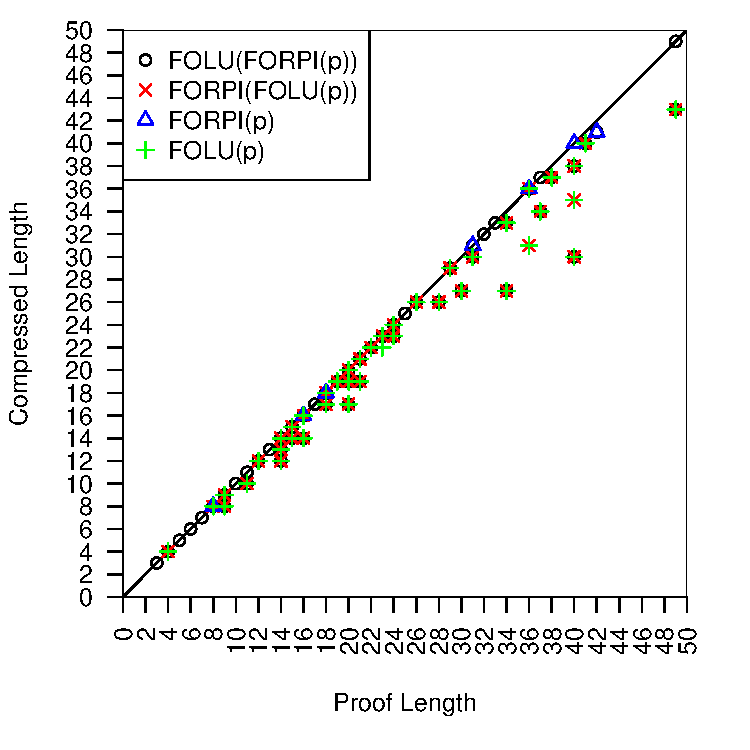
\includegraphics[scale=0.5]{images/everything-forpi-folu-length_vs_compress_length_all_proofs.pdf}}}
%    \subfloat[Compressed length against input length (resolutions)]{{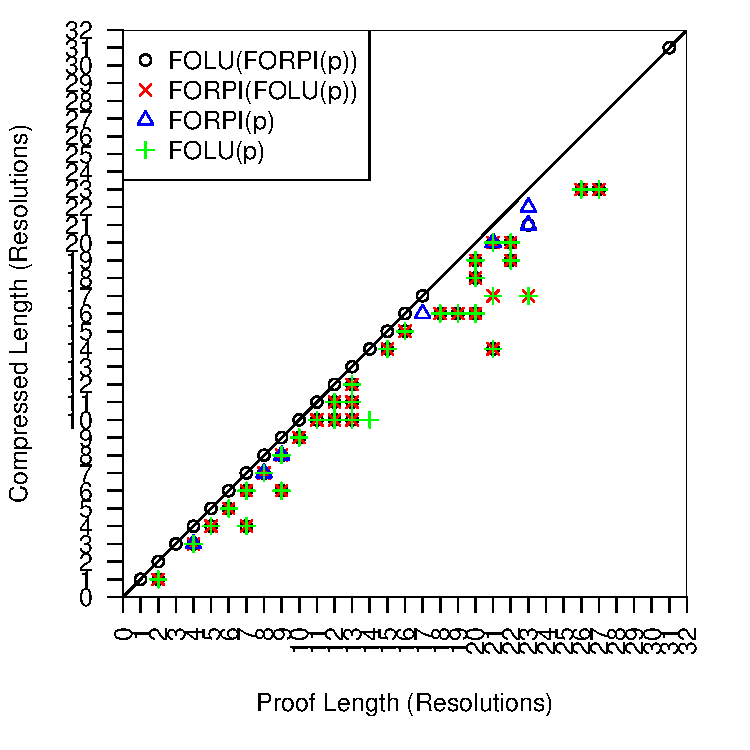
\includegraphics[scale=0.5]{images/everything-forpi-folu-res_length_vs_compress_res_length_all_proofs.pdf} }}
\subfloat[\FORPI(\GFOLU(p)) vs. \GFOLU(\FORPI(p))]{{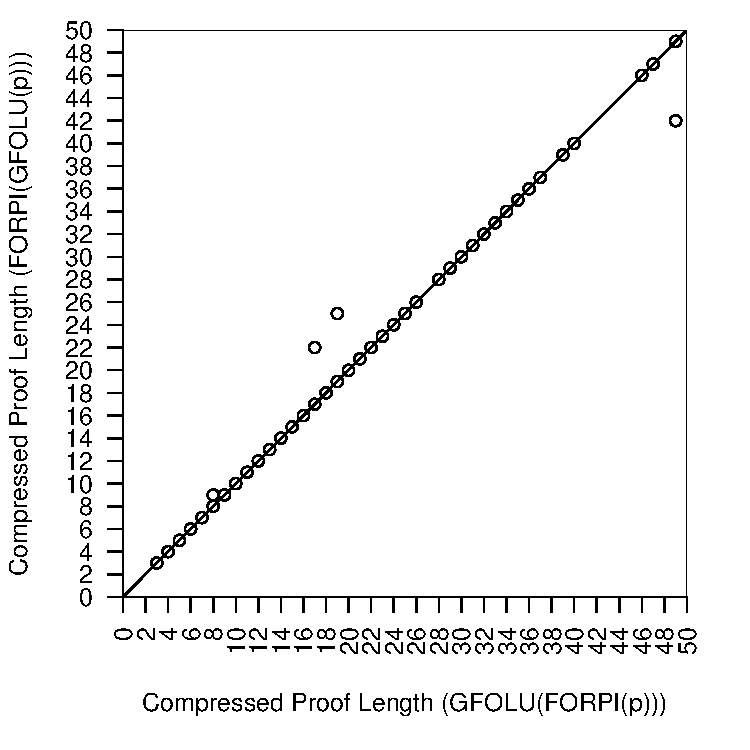
\includegraphics[scale=0.5]{images/forpi-folu-vs-folu-forpi-length_vs_compress_length_all_proofs.pdf} }}
\caption{Experimental results}
\label{fig:ex}
\end{figure}






\section{Conclusions and Future Work}

ToDo: by Bruno

{\LowerUnivalents}, the algorithm presented here, has been shown in the previous section to compress
more than {\LowerUnits}. This is so because, as demonstrated in Proposition \ref{prop:compression}, the
set of subproofs it lowers is always a superset of the set of subproofs lowered by {\LowerUnits}. It might
be possible to lower even more subproofs by finding a characterization of (efficiently) lowerable subproofs
broader than that of univalent subproofs considered here. This direction for future work promises to be challenging, though, as evidenced by the non-triviality of the optimizations discussed in Section \ref{sec:LUniv} for obtaining a linear-time implementation of {\LowerUnivalents}.



As discussed in Section \ref{sec:LUnivRPI}, the proposed algorithm can be embedded in the deletion traversal of other algorithms.  As
an example, it has been shown that the combination of {\LowerUnivalents} with {\RPI}, compared to
the sequential composition of {\LowerUnits} after {\RPI}, results in a better compression ratio with
only a small processing time overhead (Figure \ref{fig:LUnivRPI}). Other compression algorithms that also have a subproof
deletion or reconstruction phase (e.g. \ReduceReconstruct) could probably benefit from being
combined with {\LowerUnivalents} as well.

%\vspace{-10pt}
%\paragraph{Acknowledgments:}



\bibliographystyle{splncs}
\bibliography{biblio}


\end{document}

% vim: tw=100
